\documentclass[12pt]{article}
%% arXiv paper template by Flip Tanedo
%% last updated: Dec 2016



%%%%%%%%%%%%%%%%%%%%%%%%%%%%%
%%%  THE USUAL PACKAGES  %%%%
%%%%%%%%%%%%%%%%%%%%%%%%%%%%%

\usepackage{amsmath}
\usepackage{amssymb}
\usepackage{amsfonts}
\usepackage{graphicx}
\usepackage{xcolor}
\usepackage{nopageno}
\usepackage{enumerate}
\usepackage{parskip}
\usepackage{framed}
%\usepackage{bbm} 
\usepackage[normalem]{ulem}


\renewcommand{\thesection}{}
\renewcommand{\thesubsection}{\arabic{subsection}}

%%%%%%%%%%%%%%%%%%%%%%%%%%%%%%%%%%%%%%%%%%%%%%%
%%%  PAGE FORMATTING and (RE)NEW COMMANDS  %%%%
%%%%%%%%%%%%%%%%%%%%%%%%%%%%%%%%%%%%%%%%%%%%%%%

\usepackage[margin=2cm]{geometry}   % reasonable margins

\graphicspath{{figures/}}	        % set directory for figures

% for capitalized things
\newcommand{\acro}[1]{\textsc{\MakeLowercase{#1}}}    

%\numberwithin{equation}{section}    % set equation numbering
\renewcommand{\tilde}{\widetilde}   % tilde over characters
%\renewcommand{\vec}[1]{\mathbf{#1}} % vectors are boldface

\newcommand{\dbar}{d\mkern-6mu\mathchar'26}    % for d/2pi
\newcommand{\ket}[1]{\left|#1\right\rangle}    % <#1|
\newcommand{\bra}[1]{\left\langle#1\right|}    % |#1>
\newcommand{\Xmark}{\text{\sffamily X}}        % cross out

\let\olditemize\itemize
\renewcommand{\itemize}{
  \olditemize
  \setlength{\itemsep}{1pt}
  \setlength{\parskip}{0pt}
  \setlength{\parsep}{0pt}
}


% Commands for temporary comments
\newcommand{\comment}[2]{\textcolor{red}{[\textbf{#1} #2]}}
\newcommand{\flip}[1]{{\color{red} [\textbf{Flip}: {#1}]}}
\newcommand{\email}[1]{\texttt{\href{mailto:#1}{#1}}}

\newenvironment{institutions}[1][2em]{\begin{list}{}{\setlength\leftmargin{#1}\setlength\rightmargin{#1}}\item[]}{\end{list}}


\usepackage{fancyhdr}		% to put preprint number



% Commands for listings package
%\usepackage{listings}      % \begin{lstlisting}, for code
%
% \lstset{basicstyle=\ttfamily\footnotesize,breaklines=true}
%    sets style to small true-type



%%%%%%%%%%%%%%%%%%%
%%%  HYPERREF  %%%%
%%%%%%%%%%%%%%%%%%%

%% This package has to be at the end; can lead to conflicts
\usepackage{microtype}
\usepackage[
	colorlinks=true,
	citecolor=black,
	linkcolor=black,
	urlcolor=green!50!black,
	hypertexnames=false]{hyperref}





\begin{document}


\begin{center}

    {\Large \textsc{Long HW 8}:
    \textbf{Last Homework}}
    
\end{center}

\vskip .4cm

\noindent
\begin{tabular*}{\textwidth}{rl}
	\textsc{Course:}& Physics 165, \emph{Introduction to Particle Physics} (2018)
	\\
	\textsc{Instructor:}& Prof. Flip Tanedo (\email{flip.tanedo@ucr.edu})
	\\
	\textsc{Due by:}& \textbf{Tuesday}, March 6 
\end{tabular*}

\noindent
This is the main weekly homework set. Unless otherwise stated, give all responses in natural units where $c = \hbar = 1$ and energy is measured in electron volts (usually MeV or GeV). 



\subsection{Spin indices with a scalar particle}

\emph{Oh no, not this sh*t again.} You're going to want to refer back to Long HW7 problem 1. This is the same process, $e+e^- \to \mu^+\mu^-$, but this time there's an intermediate Higgs particle:
\begin{center}
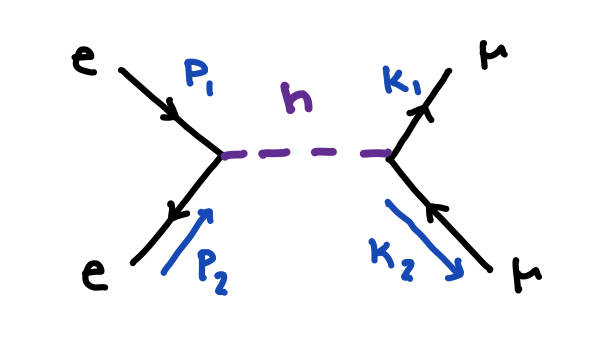
\includegraphics[width=.3\textwidth]{HW8b.png}	
\end{center}
The electron and muon are packaged into the following \textbf{Dirac spinors}:
\begin{align}
	\Psi_{(e)} &=
	\begin{pmatrix}
	e_L^\alpha
	\\
	e_R^{\dot\alpha}
	\end{pmatrix}
	&
	\Psi_{(\mu)} &=
	\begin{pmatrix}
	\mu_L^\alpha
	\\
	\mu_R^{\dot\alpha}
	\end{pmatrix} ,
\end{align}
where $e_L$ and $e_R$ are the left- and right-chiral electrons, $\mu_L$ and $\mu_R$ are the left- and right-chiral muons. Recall that the left- and right-chiral particles are totally different; for example $e_L$ is part of an SU(2) doublet field $L=(\nu_{eL}, e_L)^T$, whereas $e_R = \bar E^\dag$ doesn't know anything about SU(2). The only reason that $e_L$ and $e_R$ are stuck together is because the Higgs gave the electron mass, which means $e_L$ and $e_R$ mix quantum mechanically. 

Recall that
\begin{align}
	\gamma^0 &= 
	\begin{pmatrix}
		0 & 1_{2\times 2} \\
		1_{2\times 2} & 0 
	\end{pmatrix}
	&
	\gamma^i &= 
	\begin{pmatrix}
		0 & \sigma^i \\
		-\sigma^i & 0 
	\end{pmatrix} 
	\ .
\end{align}
In class we wrote $\sigma^0 = \bar \sigma^0 = 1_{2\times 2}$ and so that we could write 
\begin{align}
	\gamma^\mu &= 
	\begin{pmatrix}
		0 & \sigma^\mu \\
		-\bar\sigma^\mu & 0 
	\end{pmatrix} 
\end{align}
where $\bar\sigma^i = - \sigma^i$. If there's one thing you take from this class, maybe it's the observation that physicists will torture themselves with notation in order to make equations simpler.

The Higgs doublet has 2 complex components, or four real components:
\begin{align}
	H(x)^a &= 
	\begin{pmatrix}
		H_1(x) \\
		H_2(x)
	\end{pmatrix}
	=
	\begin{pmatrix}
		\hat h_1(x) + i\hat h_2(x)  \\
		h(x) + i \hat h_3(x)
	\end{pmatrix}
\end{align}
The $\hat h$ bosons are all \textit{eaten} by the massive $W^\pm$ and $Z$ bosons\footnote{Recall: a massless spin-1 has two degrees of freedom, but a massive spin-1 boson has three degrees of freedom. Thus the $W+$, $W^-$, and $Z$ each needed to `eat' a piece of the Higgs doublet to acquire this additional degree of freedom.}. The only physical particle left over is the $h$, which we call \emph{the} Higgs boson.

If we go through it, the theory of the Higgs boson talking to electrons and muons is governed by
\begin{align}
	\mathcal L 
	& = 
	\bar \Psi_{(e)} 
	i \gamma^\mu 
	D_\mu
%	\left(\partial_\mu - i e A_\mu\right) 
	\Psi_{(e)}
	+
	\bar \Psi_{(\mu)} 
	i \gamma^\mu 
%	\left(\partial_\mu - i e A_\mu\right)
	D_\mu
	\Psi_{(\mu)} 
%	- \frac 14 F_{\mu\nu}F^{\mu\nu}
	- m_{(e)} \bar \Psi_{(e)}\Psi_{(e)}
	- m_{(\mu)} \bar \Psi_{(\mu)}
	\Psi_{(\mu)}
	\\
	&
	+\frac 12(\partial_\mu h)(\partial^\mu h)
	- y_{(e)} h \bar \Psi_{(e)} 	\Psi_{(e)}
	- y_{(\mu)} h \bar \Psi_{(\mu)}  \Psi_{(\mu)} 
	\ .
\end{align}

This boils down to are the following Feynman rules:
\begin{center}
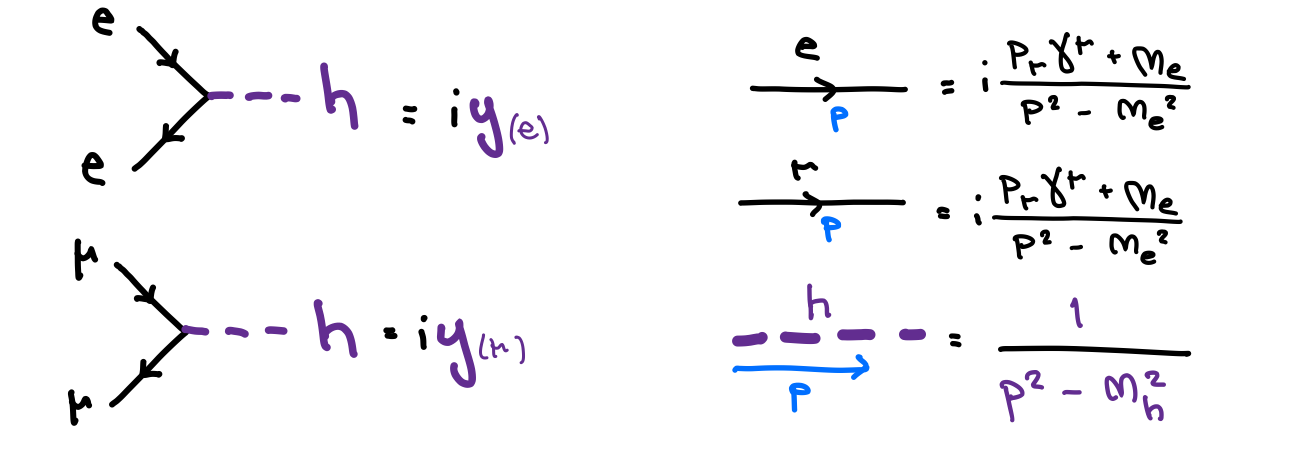
\includegraphics[width=.7\textwidth]{HW8bb.png}	
\end{center}

Putting this together, the amplitude for the $e^+e^-\to\mu^+\mu^-$ diagram above is:
\begin{align}
	y_{(e)} y_{(\mu)}\left[\bar\Psi_{(e)} \Psi_{(e)}\right] \frac{1}{(p_1+p_2)^2 - m_h^2} \left[\bar\Psi_{(\mu)} \Psi_{(\mu)}\right] \ .
\end{align}
Here $\bar\Psi = \Psi^\dag \gamma^0$. This means that
\begin{align}
	\bar\Psi &= (\psi_R^{\dag\alpha}\;,\; \psi_L^{\dag\dot\alpha}) 
	= ( \psi_R^{*\uparrow} \;,\;
	\psi_R^{*\downarrow} \;,\;
	\psi_L^{*\uparrow} \;,\;
	\psi_L^{*\downarrow} )
	&\text{for}
	&
	&
	\Psi &= (\psi_L^\alpha, \psi_R^{\dot\alpha})^T \ .
\end{align}
The terms in square brackets are matrix multiplications with respect to the spinor indices.
In this problem, you should contrast this to what happened when the intermediate particle is a photon (as we did in HW7).

Answer the following questions:
\begin{enumerate}
	%
	\item[(a)] Is this process possible when the initial states are a \emph{spin-up, left-handed electron} and a \emph{spin-up, right-handed positron}? (`Possible' means that there's a non-zero amplitude.)
	\item[(b)] Is this process possible when the initial states are a \emph{spin-up, left-handed electron} and a \emph{spin-up, left-handed positron}? 
	\item[(c)] Is this process possible when the final states are a \emph{spin-up, left-handed muon} and a \emph{spin-down, right-handed anti-muon}? 
	\item[(d)] In one sentence, what is the main difference between how a spin-0 particle like the Higgs talks to massive fermions compared to a spin-1 particle like the photon? Use the word \textbf{chirality} in your answer.
\end{enumerate}


\subsection{Standard Model on a Mug}

CERN sells mugs with the Standard Model summarized on it. It's based on a photograph of a chalkboard by John Ellis, who looks a little like Santa Claus. The mug looks like this:
\begin{center}
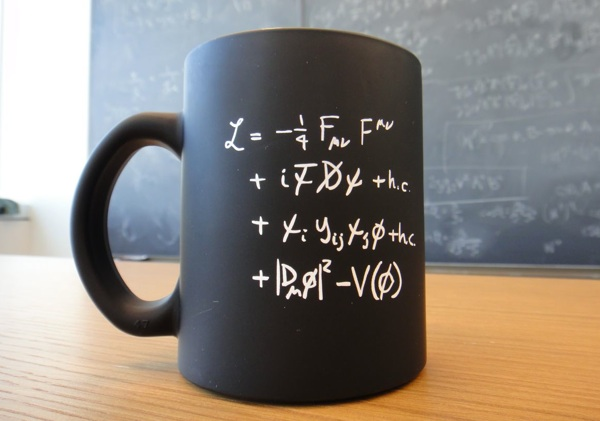
\includegraphics[width=.35\textwidth]{HW8bbb.jpg}	
\end{center}
For each term in the mug, draw a Feynman rule (a vertex, where lines come together) that comes from it. To answer this question, I urge you to read the 2017 article by Woithe et al.\footnote{\url{http://iopscience.iop.org/article/10.1088/1361-6552/aa5b25}} 

%\textsc{Answer}: you can find a discussion of the same mug in this 2010 blog post\footnote{\url{http://bit.ly/2COjSh9}}.



\subsection{Standard Model in your Life}

Read the first six sections of Robert Cahn's ``The eighteen arbitrary parameters of the standard model in your everyday life,'' available online\footnote{\url{http://dx.doi.org/10.1103/RevModPhys.68.951}}. In a few sentences, describe how the universe would differ if the Higgs boson interacted with up quarks more strongly than down quarks. \textsc{Hint}: If the Higgs talks more strongly to a particle, what does that mean for the mass of that particle?

\textsc{Extra Credit}: Pick three other parameters. In a few sentences each, describe what would happen if these parameters were very different from their values in our universe.





\appendix
\vspace{1em}
{\Large\textbf{Extra Credit}}



\subsection{Bug Bounty}

In the next week or so all of the solutions to the homework sets will be posted. The take home final exam will have problems similar to past homework, so it's in our best interest to have all of the solutions \emph{correct}. Extra credit for any corrections to the solutions ahead of the final exam. %(``Big Shot: for the Bounty Hunters.'')

\subsection{Reading}

Read Geoffrey B.\ West's article ``Scale \& Dimension: from animals to quarks!'' in \emph{Lecture Notes: from simple field theories to the standard model} in the \textit{Particle Physics: A Los Alamos Primer} collection\footnote{Link on our course website.}. What is meant by `renormalization'? (The material is remarkably subtle, but write a few sentences about what it means in plain English.)



\end{document}